\section{Preliminary model results}

\fontsize{12pt}{24pt}\selectfont We tried models based on 5 different pre-trained models - ResNet50V2, ResNet152V2, NASNetLarge, MobileNetV3Large and DenseNet121. Of these, we found the best performing to be ResNet152V2 with a training accuracy of 97.65\% and a testing accuracy of 94.42\%. We additionally measured the models on their recall, precision and F1-score. \\
Accuracy = TP + TN/TP +TN + FP + FN					-  (5.1)\\
Specificity = TN/TN + FP							-  (5.2)\\
Precision = TP/TP + FP						    	-  (5.3)\\
F1-Score = 2(Precision x Recall)/(Precision + Recall) -  (5.4)\\
where TP denotes a True Positive, TN denotes a True Negative, FP a False Positive and FN a False Negative. For this task the positive class (1) is a real image and the negative class (0) is an AI-generated image.
\begin{table}[H]
\begin{center}
\begin{tabular}{|l|l|l|l|l|}
\hline
Model & Accuracy  & Precision & Specificity & F1-Score\\ \hline
ResNet50V2   & 0.9047 & 0.9016 & 0.9032 & 0.9008         \\ \hline
ResNet152V2   & 0.9417 & 0.94285 & 0.943 & 0.9416      \\ \hline
NASNetLarge  & 0.89425 & 0.9104 & 0.9140 & 0.89211      \\ \hline
DenseNet121   & 0.90675 & 0.90332 & 0.9025 & 0.90714      \\ \hline
MobileNetV3Large   & 0.9032 & 0.91983 & 0.9230 & 0.9013      \\ \hline

\end{tabular}
\end{center}
\caption{Initial Training Results}
\end{table}

\begin{center}
   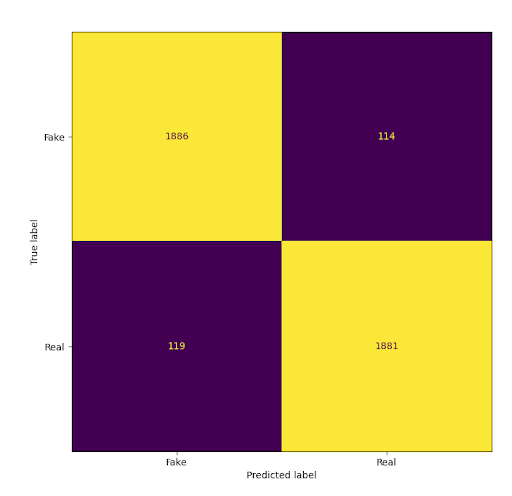
\includegraphics[width=6in, height=5in]{images/5.1.png} 
   \\\fontsize{11pt}{24pt} Figure 5.1: Confusion Matrix of best model: ResNet152V
\end{center}

	
\begin{center}
   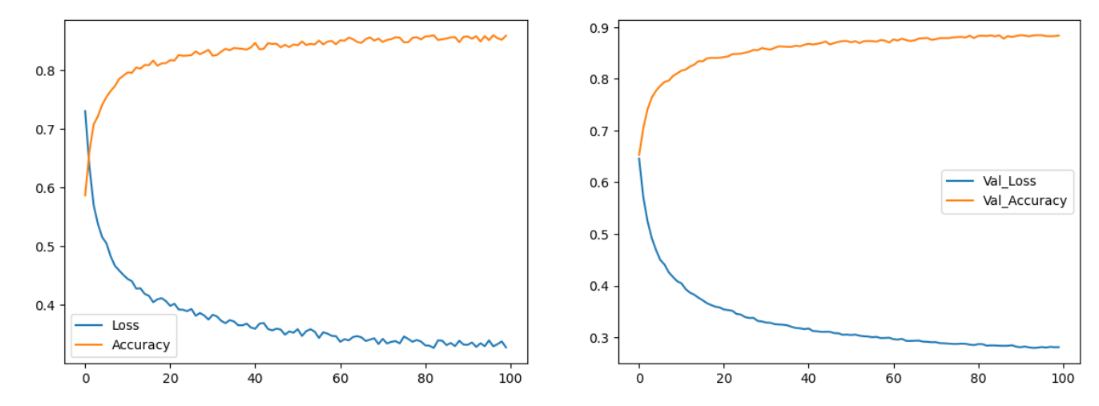
\includegraphics[width=6in, height=2.5in]{images/5.2.png} 
   \\\fontsize{11pt}{24pt} Figure 5.2: Training ResNet152V2 with top layers frozen
\end{center}

\begin{center}
   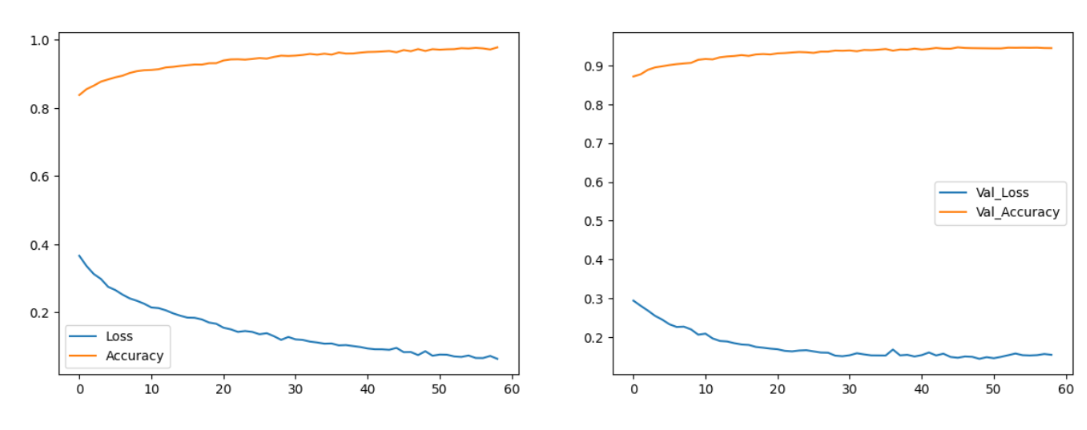
\includegraphics[width=6in, height=2.5in]{images/5.3.png} 
   \\\fontsize{11pt}{24pt}	Figure 5.3: Fine-tuning ResNet152V2 with top layers unfrozen
\end{center}


	

\section{Preliminary metaheuristic comparison}
We tried 13 metaheuristic algorithms initially- Grey Wolf Optimization and RWGWO  \cite{12} \cite{29}, Grey Wolf/Whale Optimization Hybrid  \cite{30}, PSO  \cite{10}, HPSO-TVAC  \cite{24}, Harmony Search  \cite{27}, Whale Optimization and HI-WOA  \cite{31} \cite{32}, Electromagnetic Field Optimization  \cite{33}, Genetic Algorithm and 2 other advanced variants of the GA  \cite{9} and Coral Reef Optimization  \cite{26}. We trained these algorithms using features from the MobileNetV3Large model we had previously trained. We measured only a single metric, accuracy (equation 5.1) for these algorithms. The results are presented in tabular and graphical form.

\begin{center}
   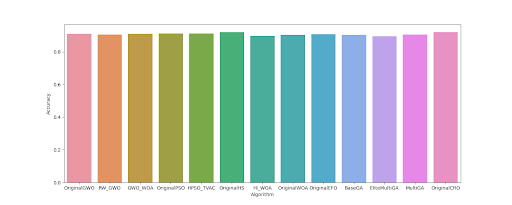
\includegraphics[width=7in, height=2.5in]{images/5.4.png} 
   \\\fontsize{11pt}{24pt}	Figure 5.4: Graphic results of metaheuristic comparison
\end{center}
\begin{table}[H]
\begin{center}
\begin{tabular}{|p{1cm}|p{4cm}|p{2cm}|}
\hline
S.No & Algorithm           & Accuracy\\ \hline
1.   & Grey Wolf Optimization & 0.9105          \\ \hline
2.   & RW-GWO      & 0.906          \\ \hline
3.   & Grey Wolf/Whale Optimization      & 0.90975          \\ \hline
4.   & PSO     & 0.913         \\ \hline
5.   & HPSO-TVAC     & 0.9125          \\ \hline
6.   & Harmony Search     & 0.9205          \\ \hline
7.   & HI-WOA     & 0.8975          \\ \hline
8.   & Whale Optimization     & 0.90375          \\ \hline
9.   & Electromagnetic Field Optimization     & 0.908          \\ \hline
10.   & Genetic Algorithm     & 0.90375          \\ \hline
11.   & Multi-Objective Elite GA     & 0.899575          \\ \hline
12.   & Multi-Objective GA     & 0.906          \\ \hline
13.   & Coral Reef Optimization     & 0.9205          \\ \hline
\end{tabular}
\end{center}
\caption{Metaheuristic Comparison}
\end{table}

We therefore use Coral Reef Optimization as our primary metaheuristic algorithm.

\section{Final Model and Metaheuristic feature selection}
We finally trained a ResNet152V2 model and used Coral Reef Optimization for feature selection, achieving an initial testing accuracy of 96.933\% after fine-tuning the model and a testing accuracy of 97.315\%. The associated training graphs and results are shown below. We calculate all relevant and previously mentioned metrics alongside a confusion matrix and an ROC curve.


\begin{center}
   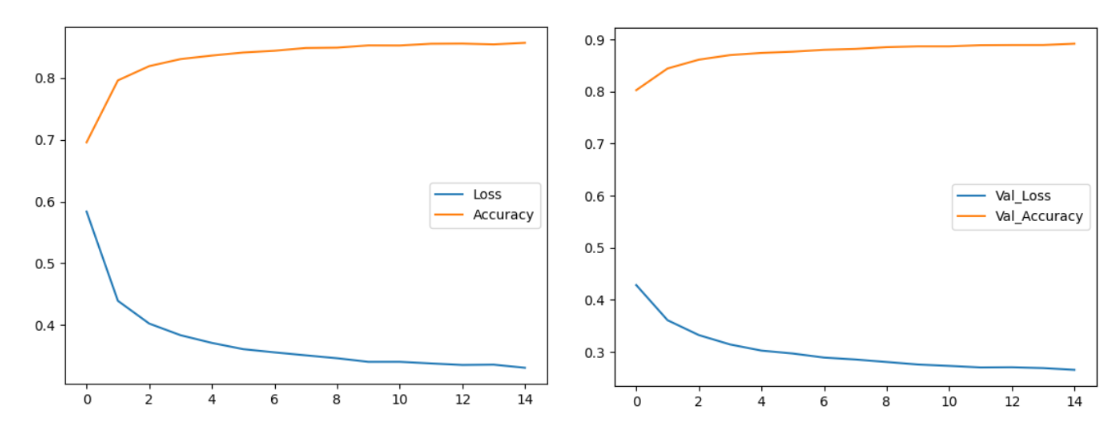
\includegraphics[width=6in, height=2.5in]{images/5.5.png} 
   \\\fontsize{11pt}{24pt}	Figure 5.5: Training the final model with top layers frozen
\end{center}


\begin{center}
   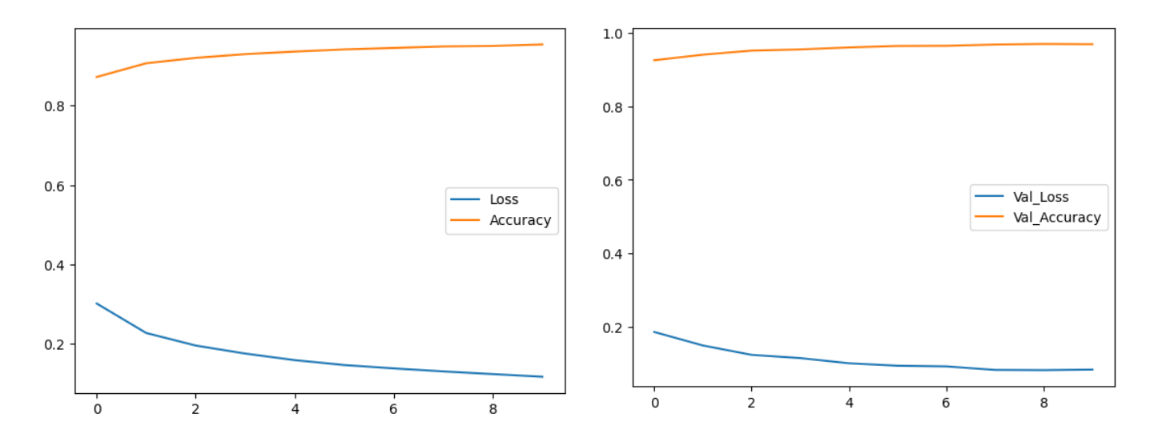
\includegraphics[width=6in, height=2.5in]{images/5.6.png} 
   \\\fontsize{11pt}{24pt}	Figure 5.6: Fine-tuning the final model with top layers unfrozen
\end{center}
			
\begin{center}
   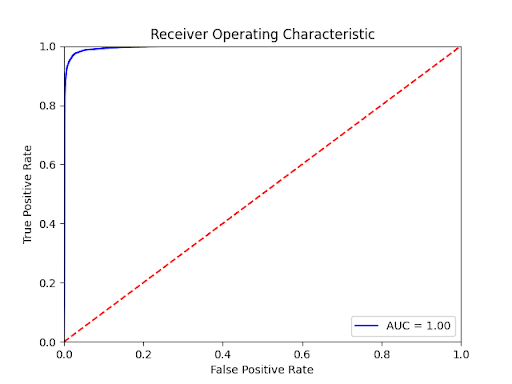
\includegraphics[width=5.5in]{images/5.7.png} 
   \\\fontsize{11pt}{24pt}	Figure 5.7: Receiver Operating Characteristic
\end{center}

\begin{center}
   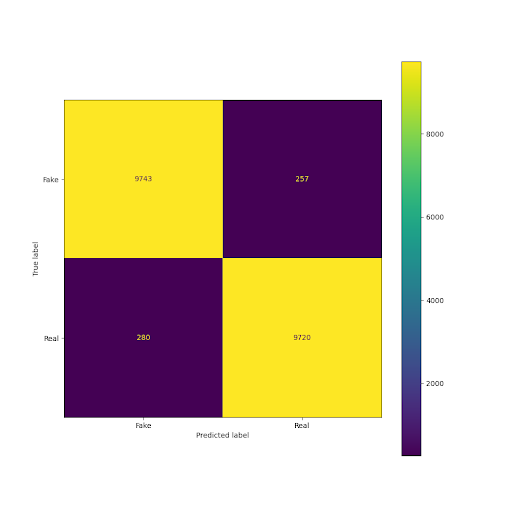
\includegraphics[width=5in,height=4in]{images/5.8.png} 
   \\\fontsize{11pt}{24pt}	Figure 5.8: Confusion Matrix for the Final Model
\end{center}
			

\begin{table}[H]
\begin{center}
\begin{tabular}{|l|l|l|}
\hline
S.No & Parameter                       & Value \\ \hline
1.   & Accuracy & 0.97315          \\ \hline
2.   & Specificity      & 0.9743          \\ \hline
3.   & Precision      & 0.97424          \\ \hline
4.   & F1-Score     & 0.97311          \\ \hline
5.   & ROC-AUC Score     & 0.99571          \\ \hline

\end{tabular}
\end{center}
\caption{Final Results}
\end{table}


		




